\chapter{Variational Bayesian Approximation
via $D_{KL}$}

For more info and references about
this topic, see Ref.\cite{wiki-var-bay}.

A Variational Bayesian Approximation (VBA)
is when we approximate
a probability distribution
by another 
probability distribution that depends
on a continuous \qt{variational parameter}.
This parameter is
adjusted 
within its range of possible values,
to make the approximation
as good as possible.
There are many VBA methods.
VBA methods are inspired by 
ancient  methods
used in Calculus 
of Variations applied to Physics
and Engineering problems.

In this chapter, we do VBA via 
the Kullback-Leibler divergence $D_{KL}$.
We approximate the probability 
distribution $P(h|\vecx)$,
where $h$ are the hidden variables 
and $\vecx$ is the data. 
More precisely, suppose $\rvh\in S_\rvh$ and $\rvq\in S_\rvh$.
Suppose $\vec{\rvx}\in S_\rvx^{nsam}$
 is a vector of $nsam$ samples
and the samples $\rvx[\sigma]\in S_\rvx$ are i.i.d..
 The VBA is simply 
an approximation
$P_{\rvq|\vec{\rvx}}$ to
$P_{\rvh|\vec{\rvx}}$:


\beq
P_{\rvh|\vec{\rvx}}(h|\vecx)
\approx P_{\rvq|\vec{\rvx}}(h|\vecx)
\eeq
obtained by minimizing the Kullback-Leibler divergence
$D_{KL}(P_{\rvq|\vec{\rvx}}\parallel
P_{\rvh|\vec{\rvx}})$
over all 
$P_{\rvq|\vec{\rvx}}$. The minimization
is 
usually subject to some constraints
on the admissible forms of 
$P_{\rvq|\vec{\rvx}}$.


$D_{KL}(Q\parallel P)\neq
D_{KL}(P\parallel Q)$; i.e.,  $D_{KL}$ is not
symmetric. So why do we use 
$D_{KL}(P_{\rvq|\vec{\rvx}}\parallel
P_{\rvh|\vec{\rvx}})$
instead of 
$D_{KL}(
P_{\rvh|\vec{\rvx}}\parallel P_{\rvq|\vec{\rvx}})$?
Because 
$D_{KL}(
P_{\rvh|\vec{\rvx}}\parallel P_{\rvq|\vec{\rvx}})$
requires knowledge of $P_{\rvh|\vec{\rvx}}$,
but calculating $P_{\rvh|\vec{\rvx}}$
is what we are trying to do in the first place.

\begin{figure}[h!]
\centering
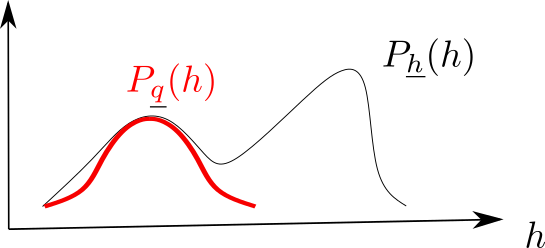
\includegraphics[width=2.5in]
{var-bay/kl-q-support.png}
\caption{
If $P_\rvq(h)$
is Gaussian shaped 
and $P_\rvh(h)$
has multiple
bumps (modes)
then 
$D_{KL}(P_\rvq\parallel P_\rvh)$
is minimized when $P_\rvq$
fits one of the modes of $P_\rvh$.
That is because $D_{KL}(P_\rvq\parallel P_\rvh)=
\sum_h P_\rvq(h)\ln \frac{P_\rvq(h)}{P_\rvh(h)}$
is a weighted average with weights $P_\rvq$,
so nothing going on outside the support
of $P_\rvq$ influences  much
the final average.
}
\label{fig-kl-q-support}
\end{figure}


See Fig.\ref{fig-kl-q-support}
for some intuition
on what minimizing
$D_{KL}(P_{\rvq|\vec{\rvx}}\parallel
P_{\rvh|\vec{\rvx}})$ means.


\begin{figure}[h!]
$$\xymatrix{
& \rvh_0\ar[r]
& \rvh_1
\\
\rvx[0]
\ar[ru]\ar[rru]
\ar[rddd]\ar[rrddd]
\\
\rvx[1]
\ar[ruu]\ar[rruu]
\ar[rdd]\ar[rrdd]
\\
\rvx[2]
\ar[ruuu]\ar[rruuu]
\ar[rd]\ar[rrd]
\\
&
\rvq_0
&
\rvq_1
}$$
\caption{
$\rvq$ 
and $\rvh$ have  $nh=2$
mirroring components and
those of $\rvq$ are independent
at fixed $\vec{\rvx}$.}
\label{fig-q-apes-h}
\end{figure}


Suppose $\rvh=(\rvh_0, \rvh_1, \ldots, \rvh_{nh-1})$
and
$\rvq=(\rvq_0, \rvq_1, \ldots, \rvq_{nh-1})$
where $\rvh_i\in S_{\rvh_i}$
and $\rvq_i\in S_{\rvh_i}$ for all $i$.
We say $\rvq$ 
and $\rvh$ have  $nh$ mirroring
 components and
those of $\rvq$ are independent
at fixed $\vec{\rvx}$ if

\beq
P_{\rvq|\vec{\rvx}}(h|\vecx)
=\prod_i P_{\rvq_i|\vec{\rvx}}(h_i|\vecx)
\;.
\eeq
The bnet Fig.\ref{fig-q-apes-h}
describes the scenario that
we have in mind: The samples 
$\rvx[\sigma]$ are i.i.d..
Each component $\rvh_i$
of $\rvh$ has a 
mirroring
component $\rvq_i$
in $\rvq$.
The components of
$\rvh$ are correlated
whereas those of $\rvq$
are independent
at fixed $\vec{\rvx}$.

\begin{claim}
If $\rvq$
and $\rvh$ 
 have $nh$ mirroring components 
and those of $\rvq$ are independent
at fixed $\vec{\rvx}$ and
$D_{KL}(P_{\rvq|\vec{\rvx}}\parallel
P_{\rvh|\vec{\rvx}})$
is minimum
 over all $P_{\rvq|\vec{\rvx}}$, then

\beqa
P_{\rvq_i|\vec{\rvx}}(q_i|\vecx)
&=&
\caln(!q_i)
e^{
E_{(\rvq_j)_{j\neq i}}[
\ln P_{\rvh| \vec{\rvx}}(\rvh=q|\vecx)]
}
\label{eq-fixed-vecx}
\\
&=&
\caln(!q_i)
e^{
E_{(\rvq_j)_{j\neq i}}[
\ln P_{\rvh, \vec{\rvx}}(\rvh=q, \vecx)]}
\;
\eeqa
for all $i$.
\end{claim}
\proof

Since all quantities in Eq.(\ref{eq-fixed-vecx})
are conditioned on $\vecx$, let 
us omit all mention of 
$\vecx$ in this proof.

Let

\beq
\call= \call_0 + \call_1
\eeq
where

\beqa
\call_0
&=&
D_{KL}(P_{\rvq}\parallel P_{\rvh})
\\
&=&
\sum_h P_\rvq(h)\ln \frac{P_\rvq(h)}{P_\rvh(h)}
\\
&=&
\sum_h P_{\rvq}(h)\ln P_\rvq(h)
- \sum_h P_{\rvq}(h)\ln P_\rvh(h)
\\
&=&
\sum_i \sum_{h_i}
 P_{\rvq_i}(h_i)\ln P_{\rvq_i}(h_i)
- \sum_h P_{\rvq}(h)\ln P_\rvh(h)
\eeqa
and

\beq
\call_1=
\sum_i \lam_i \left[
\sum_{h_i}P_{\rvq_i}(h_i)-1\right]
\;.
\eeq
Then   

\beq
\delta \call=
\sum_i
\sum_{h_i}
\delta P_{\rvq_i}(h_i)
\left[
\ln P_{\rvq_i}(h_i)
+1 + \lam_i
-\;\frac{1}{nh}\sum_{(h_j)_{j\neq i}}
\prod_{(h_j)_{j\neq i}}
\{P_{\rvq_j}(h_j)\}\ln P_\rvh(h)
\right]
\;.
\eeq
Hence,

\beq
P_{\rvq_i}(h_i)
=
\caln(!h_i)
e^{
\sum_{(h_j)_{j\neq i}}
\left\{\prod_{(h_j)_{j\neq i}}
P_{\rvq_j}(h_j)\right\}\ln P_\rvh(h)
}
\;.
\eeq
\qed

Note that 
Eq.(\ref{eq-fixed-vecx})
yields
a  system
of $nh$ nonlinear equations
in $nh$ unknowns
$(P_{\rvq_i|\vec{\rvx}})_
{i=0, 1, \dots, nh-1}$.
This system 
is usually solved recursively.


\section{Free Energy $\calf(\vecx)$}

To simplify the notation
below, let us
introduce
the following
abbreviations:

\beq
P(h|\vecx)=P_{\rvh|\vec{\rvx}}(h| \vecx)
\eeq

\beq
P(h,\vecx)=P_{\rvh,\vec{\rvx}}(h, \vecx)
\eeq

\beq
P(\vecx)=P_{\vec{\rvx}}(\vecx)
\eeq

Note that

\beqa
D_{KL}(P_{\rvq|\vec{\rvx}}\parallel
P_{\rvh|\vec{\rvx}})&=&
\sum_h P_{\rvq|\vec{\rvx}}(h|\vecx)\ln
 \frac{P_{\rvq|\vec{\rvx}}(h|\vecx)}{P(h|\vecx)}
\\
&=& \sum_h P_{\rvq|\vec{\rvx}}(h|\vecx)\ln
 \frac{P_{\rvq|\vec{\rvx}}(h|\vecx)}{P(h,\vecx)}
+ \ln P(\vecx)
\\
&=&
\calf(\vecx)+ \ln P(\vecx)
\eeqa
Hence, the {\bf Free energy} $\calf(\vecx)$
 is defined as

\beqa
\calf(\vecx)&=&
\sum_h P_{\rvq|\vec{\rvx}}(h|\vecx)\ln
 \frac{P_{\rvq|\vec{\rvx}}(h|\vecx)}{P(h,\vecx)}
\\
&=&
E_{\rvq|\vec{\rvx}}\left[
\ln
 \frac
{P_{\rvq|\vec{\rvx}}(q|\vecx)}
{P_{\rvh, \vec{\rvx}}(q,\vecx)}
\right]
\;.
\eeqa
The name free energy is justified because

\beq 
\calf(\vecx)=
\underbrace{-\sum_h P_{\rvq|\vec{\rvx}}(h|\vecx)\ln
P_{\rvh, \vec{\rvx}}(h,\vecx)}_
{U, \text{ Internal Energy}}
+
\underbrace{\sum_h P_{\rvq|\vec{\rvx}}(h|\vecx)
\ln P_{\rvq|\vec{\rvx}}(h|\vecx)}_
{-S, \text{ minus Entropy}}
\;.
\eeq

It is also common to define a
quantity called \qt{ELBO} to be the negative
of the free energy.

\beq
ELBO(\vecx)=-\calf(\vecx)
\eeq
ELBO stands for \qt{Evidence Lower BOund}.
That name
is justified because

\beq
\underbrace{\ln P_{\vec{\rvx}}(\vecx)}
_{\text{evidence} \leq 0}
=
\underbrace{D_{KL}(P_{\rvq|\vec{\rvx}}\parallel
P_{\rvh|\vec{\rvx}})}_{\geq 0}
-|ELBO(\vecx)|
\;.
\eeq

\begin{figure}[h!]
\centering
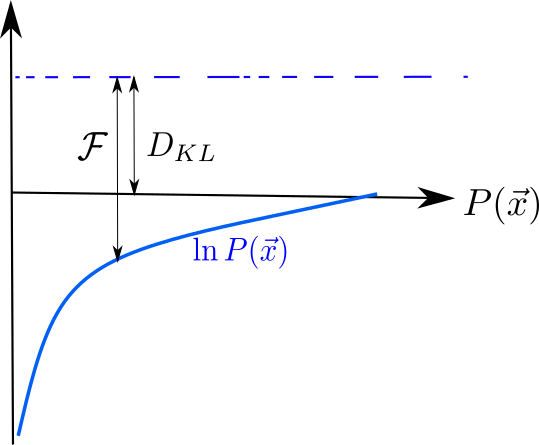
\includegraphics[width=2in]
{var-bay/elbo.png}
\caption{
$D_{KL}+\ln \frac{1}{P(\vecx)}=\calf$.
}
\label{fig-elbo}
\end{figure}

Some properties of $\calf$ are:
\begin{itemize}

\item{\bf  $\calf$ is non-negative.}

\beq
\underbrace{D_{KL}(P_{\rvq|\vec{\rvx}}\parallel 
P_{\rvh|\vec{\rvx}})}_{\geq 0}
+ \underbrace{\ln\frac{1}
{ P_{\vec{\rvx}}(\vecx)]}}_{\geq 0}
= \calf(\vecx)
\eeq



\item {\bf KL divergence is  min  iff $\calf$ is min
at fixed $P(\vecx)$.}

During a variation $\delta$ that holds
$P(\vecx)$ fixed, 
the KL divergence and $\calf$ change
by the same amount:

\beq
\delta D_{KL}(P_{\rvq|\vec{\rvx}}\parallel
P_{\rvh|\vec{\rvx}})
=
\delta \calf(\vecx)
\eeq

\end{itemize}



